
This chapter will discuss basic univariate analysis and summary statistics from the survey results, alongside what
could be inferred from these. We will look at each section individually and perform multiple initial comparisons
whereby we subset for various factors, such as degree subject, the language used to make the plots, and the order
in which plots have been presented.

\section{American Ninja Warrior, Part 1 - Y-Scaling}
The purpose of this set of questions was to decipher whether altering the type of y-scaling used would notably affect perception of the data, in 
terms of both gauging exact values as well as giving subjective opinions on differences between values. As described previously, the set of questions in the first section is as follows:

\begin{itemize}
    \item \textbf{Q1 - "Approximately many times would you say the 'Salmon Ladder' was used?"}
    \item \textbf{Q2 - "Approximately how much more than 'Log Grip' would you say 'Salmon Ladder' was used?"}
    \item \textbf{Q3 - "Approximately how much more than 'Quintuple Steps' would you say 'Salmon Ladder was used?"}
    \item \textbf{Q4 - "In your opinion, approximately how many times would you say 'Log Grip' was used, as a percentage of the number of times 'Salmon Ladder' was used?"}
\end{itemize}

First we will look at the summary statistics for each of the four questions laid out above for the whole population, before subsetting for language, degree subject, and survey version number. Each table of summary statistics presents columns for the three plot types; the control plot, the truncated plot, and the log-scaled plot, respectively in that order.

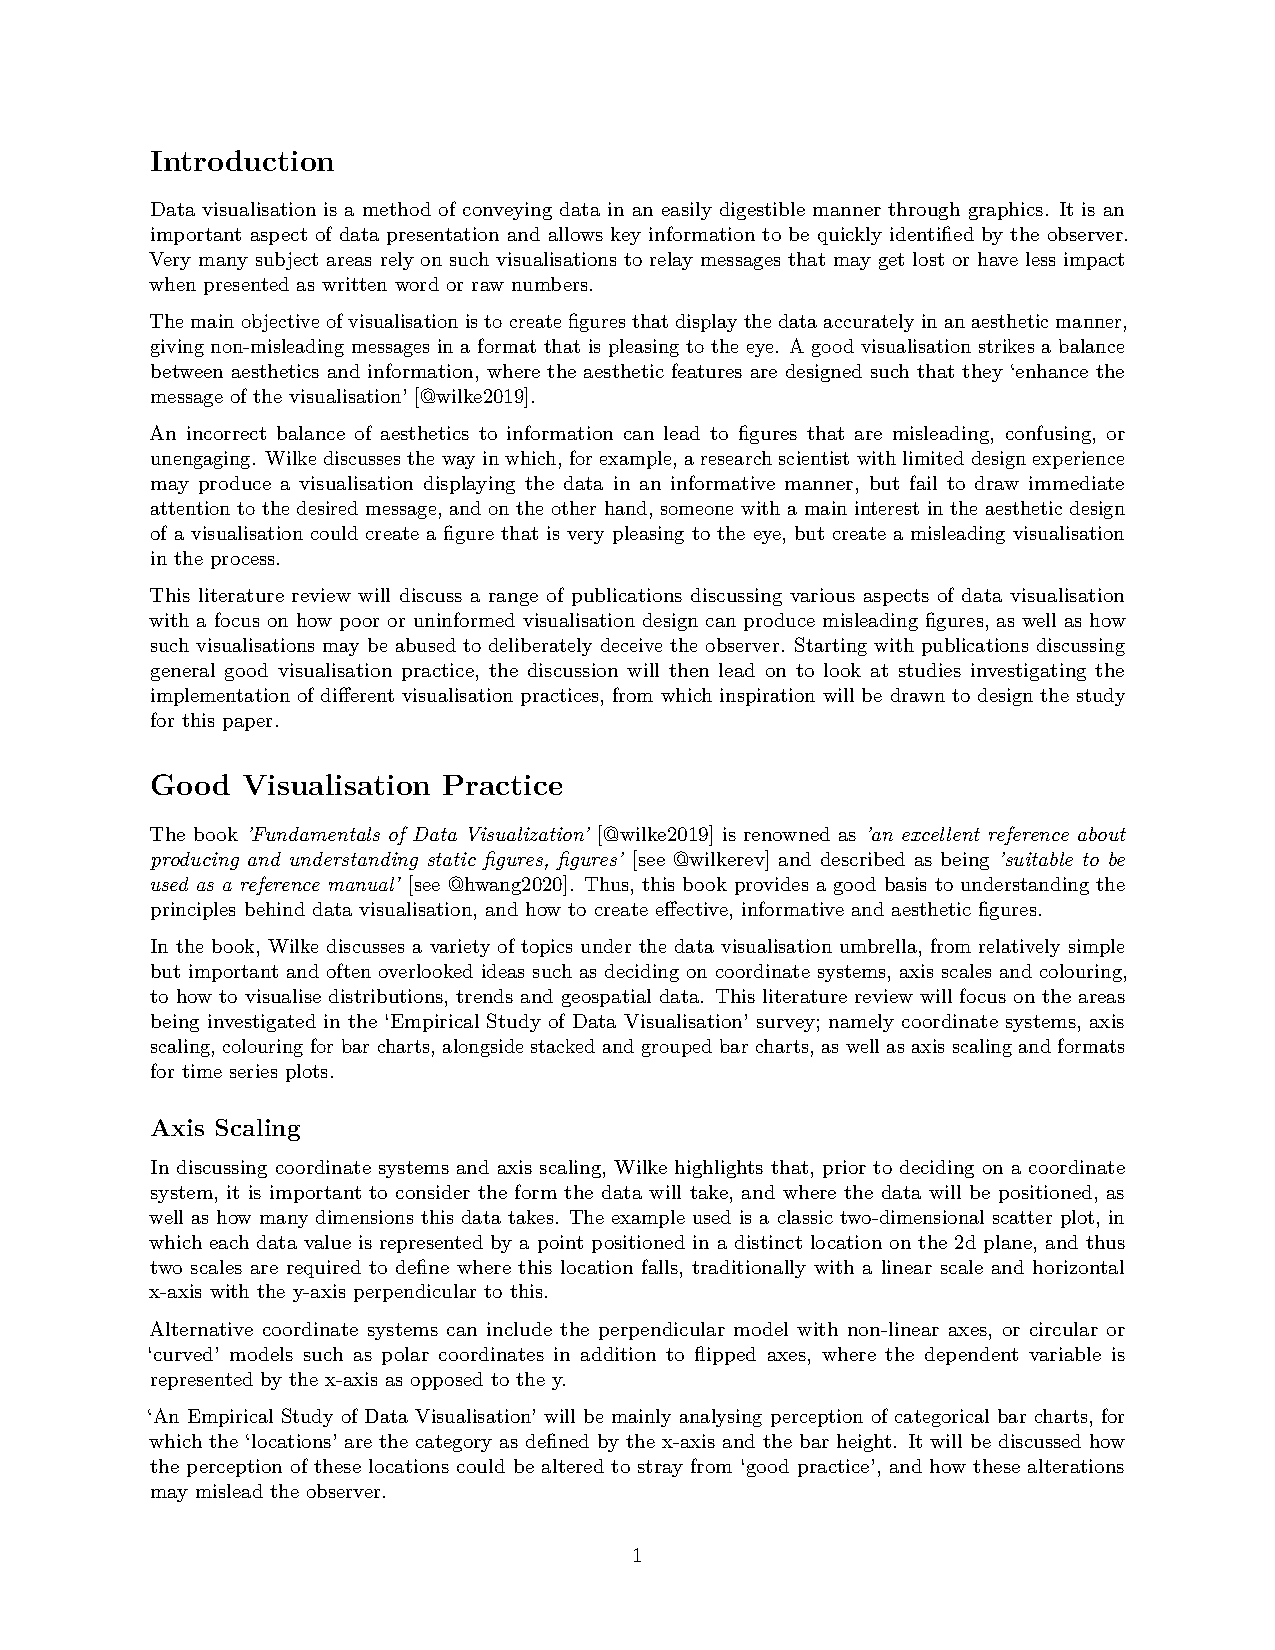
\includepdf[pages=-, pagecommand={}]{C:/Users/Katie/OneDrive/Uni_Work_Year4/Project/Year-4-Project/src/R/univariate-analysis/Section-1/Whole-pop/main.pdf}












